\documentclass{article}
\usepackage[T1]{fontenc}

\usepackage{graphicx}
\usepackage{listings}
\begin{document}

\title{FOSS Lab Report}
\author{Gokul K\\[2\baselineskip]
Roll Number: 21\\[2\baselineskip]}
\date{06 February 2020}

\maketitle

\setcounter{section}{22}
\section{Awk Scripting IV}
\subsection{Aim}
Write an awk script to compute gross salary of an employee accordingly to
rule given below : If basic salary < 10000 then DA = 45\% of the basic and 
HRA =15\% of basic If basic salary >= 10000 then DA =50\% of the basic and 
HRA =20\% of basic.


\subsection{Source Code}
\begin{verbatim}
#! /bin/awk -f

# Write an awk script to compute gross salary of an employee accordingly to
# rule given below : If basic salary < 10000 then DA = 45% of the basic and 
# HRA =15% of basic If basic salary >= 10000 then DA =50% of the basic and 
# HRA =20% of basic.

BEGIN{
    print "Employee\tGross Salary"
    print "---------------------"
}

{
    if($2 < 10000){
        totalAllowance = $2*(0.45) + $2*(0.15)
        print $1 "\t\t" totalAllowance+$2
    }

    else{
        totalAllowance = $2*(0.50) + $2*(0.20)
        print $1 "\t\t" totalAllowance+$2
    }    

}
\end{verbatim}

\subsection{Output}
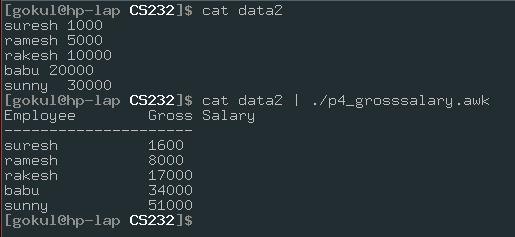
\includegraphics[width=0.9\textwidth]{img/p23.png}\newline

\subsection{Result}
The above program is run on Manjaro Linux running GNU Awk 5.0.1. 
Each query is checked and output is verified
\end{document}